 \subsection{PRISM}
 PRISM is a probabilistic model checker allowing formal modelling and analysis of systems that exhibit random or probabilistic behaviour. In our case, we will use PRISM to model a Continuous-Time Markov Chain (CTMCs) but there are other models that can be be modeled thanks to this tool. \\
 Thanks to PRISM, we will for example be able to show that every traffic lights will get the green light in an equal and fair way, meaning that there will be no starvation for one of them. Moreover, thanks to PRISM, we can show the statistics of green light possession for every different traffic light, something that is not possible to do in Uppaal. This is why we decided to also rewrite our model in PRISM so new kind of properties could be demonstrated.
 \begin{figure}[h]\label{fig:prism}
  \begin{center}
    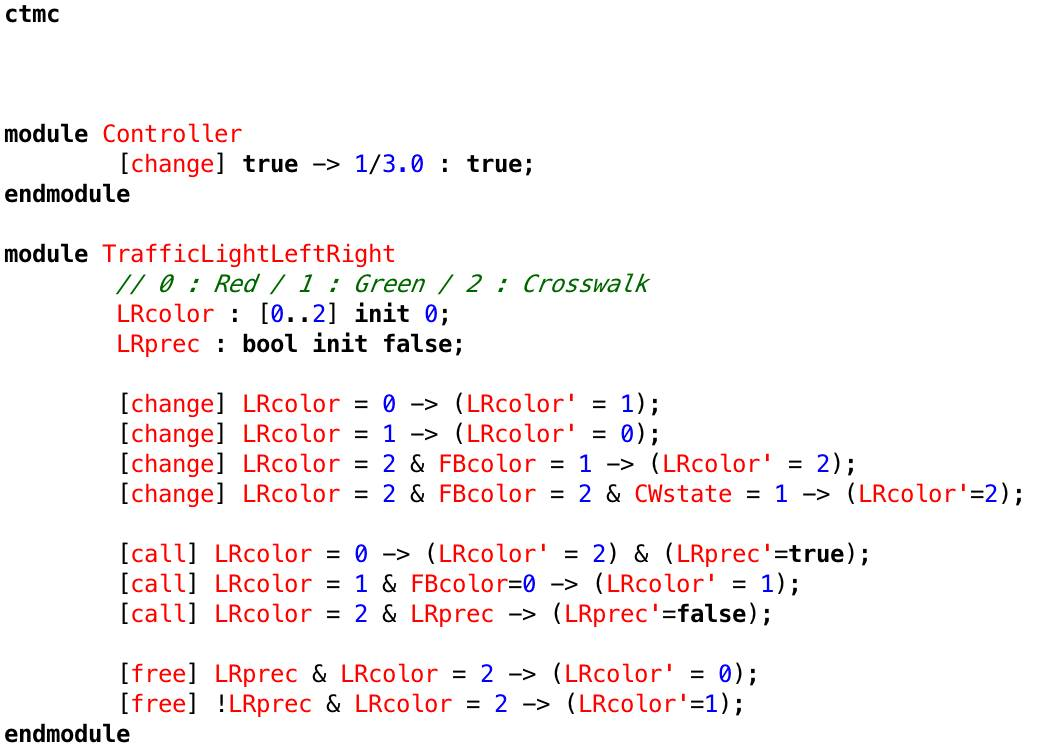
\includegraphics[width=0.8\textwidth]{picture/prism.png}
    \caption{Example of the PRISM language}
  \end{center}
\end{figure} 

\noindent In this basic code, we can already see how the syntax works in PRISM. We first define that our model will follow a Continuous-Time Markov Chain by writing ctmc as first line. We then define what PRISM call \textit{module} and it is the same that what we called \textit{Template} in Uppaal. There, we will define our Controller, our different traffic lights and so on. \\
We can communicate through the different module thanks to the labels we put between brackets and every component with the same label will be executed at the same time, once. \\
One problem with PRISM and our project is that we want the traffic lights to change every T seconds. This is something that cannot really be done in PRISM, at short-term. Indeed, even if we define a rate, systems transitions can still happen even if $T' \ne T $. This will be solved by looking at how our system works in long-term and in a long-run. Indeed, the rate that is defined by our controller will be reach T when the number of executions is high. \\ 
This is why we can use PRISM and we will use it to demonstrate other properties that cannot be shown in Uppaal.
